\chapter{Map design and generation framework}

% INTRODUCTION %

In this chapter we describe the \<framework> that we have developed to study the design and generation of maps for multiplayer Firsts Person Shooters. After a quick overview, we present the map formats that the framework supports and we extensively analyze its structure, its components and its features.

% DESCRIPTION %

\section{Description of the framework}

We designed our framework with the objective of providing a valid alternative to the games currently employed as a tool in this research field. All the available options, like \<Cube 2: Sauerbraten>, are powerful tools to perform studies involving artificial agents, but they are not suitable for user-based studies. A data-collection campaign based on these games requires either downloading the game or taking part in real-life play-test sessions, but these options discourage potential participants because they are significantly time-consuming. For this reason, we decided to develop a \<Unity>\footnote{Unity Technologies, 2005. \<Unity> is a game development environment that includes a game editor and a game engine. Currently, it is the most used game development tool.} framework that is as light as possible, with a WebGL build weighting less than 10MB that can be played using any browser.

\par

Since the purpose of this tool is to be used in research, we decided to support most map representation formats used in previous works and we designed our framework to be as modular, expansible and configurable as possible.

% SUPPORTED REPRESENTATION %

\section{Map representation}

Maps are structured as grids of orthogonal \<tiles> and are internally represented  by matrices of characters, where each cell corresponds to a specific \<tile>. Depending on the character it contains, a cell can represent a wall, a floor or an object on the floor. If a cell corresponds to a wall tile we say it is \<filled>, if it corresponds to a floor tile we say it is \<empty>. The framework supports multi-level maps, which are represented by a list of matrices, with each matrix corresponding to a level.

\par

The framework allows to represent maps in two more formats, that are converted to the internal one when provided as input.

% FILE %

\subsection{Text representation}

The text representation allows to encode the map as a text, of which each line corresponds to a row of the internal matrix representation and each character corresponds to a cell. For multi-level maps, the format is the same, with the exception of blank lines used to separate the floors, that are encoded from the lower one to the higher one.

% ALL-BLACK %

\subsection{All-Black representation}

Our All-Black representation is an extended version of the one defined by Cardamone et al.\cite{Cardamone:2011:EIM:2008402.2008411}, to which we have added the support for objects and multi-level maps. In their work, the All-Black representation encodes the empty areas of an otherwise filled map, consisting in square rooms and corridors of fixed width. Rooms are defined by $\langle x,y,s \rangle$ triplets, where $x$ and $y$ define the coordinates of the center of the room and $s$ defines its width. Corridors are rectangular areas with a fixed width of $3$ cells and are defined by $\langle x,y,l \rangle$ triplets, where $x$ and $y$ define the point in which the corridor starts and $l$ defines its length. $l$ also provides the direction of the corridor: if $l$ is positive the corridor extends along the $x\text{-axis}$, otherwise it extends along the $y\text{-axis}$. With respect to this representation, we changed the encoding of the rooms by considering $x$ and $y$ as the coordinates of the corner closer to the origin; this change allows to remove any ambiguity deriving from the position of the center of a room of even width.

\par

For allowing the encoding of objects, we added a third kind of triplet, $\langle x,y,o \rangle$, that uses $x$ and $y$ to denote the coordinates of the tile that hosts the objects and $o$ to denote the object itself, encoded as a character. In our representation, first we store the triplets representing the rooms, then the triplets representing the corridors and finally the triplets representing the objects. These groups are separated by the special character ``$\mid$'' and can have any number of elements, with the exception of the one denoting the rooms, that must have at least one triplet.

\par

We have also extended the All-Black representation including the one defined by Cachia et al.\cite{MultiLevelEvolution}, that allows to encode maps generated with a random digger algorithm, i.e. an algorithm that randomly moves in a filled map emptying all the cells it crosses (for more details see subsubsection \ref{sssec:digger}). The map is encoded by a quintuple $\langle f,l,r,v,s \rangle$, where $f$ encodes the probability of moving forwards, $l$ encodes the probability of turning left, $r$ encodes the probability of turning right, $v$ encodes the probability of jumping to a visited cell and $s$ encodes the probability of placing a flight of stairs, if in a multi-level setting. With respect to the representation defined by Cachia et al., we added the possibility of encoding objects, which group of triplets is separated by the digger quintuple by the special character ``$\mid$''.

\par

Multi-level maps are represented by encoding the floors from the lower one to the higher one using one of the two single-level All-Black formats that we have defined. The encoding of different floors are separated using the double special characters ``$\mid\mid$''.

\par

Figure \ref{fig:allblack} shows two maps with their All-Black representation.

\begin{figure}[tp]
	\centering
	\hfill
  	\begin{subfigure}[t]{0.45\linewidth}
		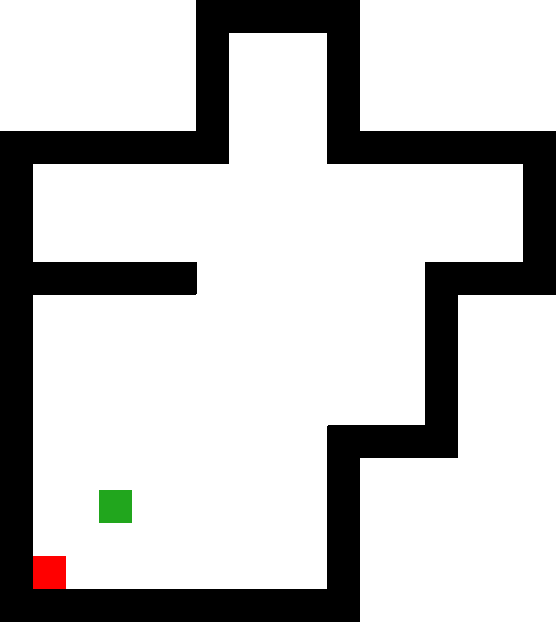
\includegraphics[width=\linewidth]{ab_divisive_1}
     		\caption{Map represented by $\langle 5, $\ $ 5, $\ $ 9 \rangle $\ $ \langle 10, $\ $ 10, $\ $ 7 \rangle $\ $  \langle 15, $\ $ 25, $\ $ 3 \rangle\ $\ $ \mid $\ $  \langle 5, $\ $ 15, $\ $ 15 \rangle $\ $  \langle 11, $\ $ 15, $\ $ -7 \rangle $\ $  \mid $\ $  \langle 5, $\ $ 5, $\ $ s \rangle $\ $  \langle 7, $\ $ 7, $\ $ d \rangle$.}
 	\end{subfigure}
 	\hfill
  	\begin{subfigure}[t]{0.45\linewidth}
    		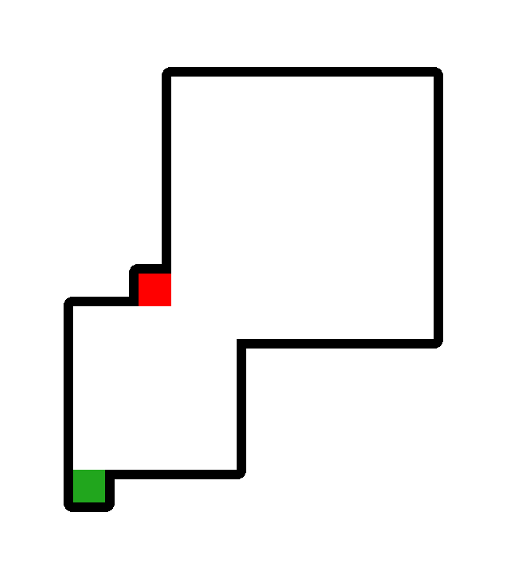
\includegraphics[width=\linewidth]{ab_divisive_2}
     		\caption{Map represented by $\langle 1,$\ $2, $\ $5  \rangle $\ $\langle4,$\ $6,$\ $8\rangle $\ $ \mid $\ $ \langle5,$\ $6,$\ $-10\rangle $\ $ \langle10,$\ $15,$\ $-6\rangle $\ $ \mid $\ $ \langle3, $\ $7, $\ $s\rangle $\ $ \langle1, $\ $1, $\ $d\rangle$.}
  	\end{subfigure}
  	\hfill
\caption{Two simple maps with their All-Black representation.}
\label{fig:allblack}
\end{figure}

% FRAMEWORK STRUCTURE % 

\section{Framework structure}

The framework collects data by assigning to the users \<matches> to play. A match is defined by the \<game mode> and by the \<map type>, which in turn is defined by the \<map topology> and by the \<map appearance>. The \<map topology> defines how the map is going to \<be> and depends on the algorithm used to generate it, whereas the \<map appearance> defines how the map is going to \<look> and depends on how the map is assembled. This implies that the map type defines a whole array of procedurally generated maps that share the same topology and appearance. Therefore, when referring to a match we are considering a specific game-mode played in a procedurally generated map. If needed, it is possible to use a pre-generated map instead of generating a new one, by providing it as input using one of the supported formats. In this case the \<map topology> defines how to interpret the input, that is then displayed considering the \<map appearance>.

\par

A match is defined by combining different modules, called \<Managers>, each of which controls a different aspect of the match.

% GAME MANAGER %

\subsection{The Game Manager}

The \<Game Manager> is the module responsible for the overall behavior of a match. Each game mode consists in a different version of the \<Game Manager>. It leans on the \<Map Manager> for the generation and the assembly of the map and on the \<Spawn Point Manager> for the spawn of entities. The \<Game Manager> controls the life-cycle of the match, that can be divided in the following phases:

\begin{itemize}
\item \<Setup>: all the modules are initialized.
\item \<Generation>: the \<Map Manager> generates or imports the map and assembles it.
\item \<Ready>: the \<Game Manager> displays a countdown announcing the start of the game.
\item \<Play>: the \<Game Manager> handles the game while the \<Experiment Manager> logs the actions of the player, if needed. This phase continues until an end condition is satisfied.
\item \<Score>: the \<Game Manager> stops the game and displays the final score.
\end{itemize}

% MAP MANAGER %

\subsection{The Map Manager}

The \<Map Manager> controls the generation, the import and the assembly of the map and the displacement of objects inside it. It leans on the \<Map Generator> for the generation, on the \<Map Assembler> for the \<assembly>\footnote{With \<assembly> we mean the operation of creating a 3D model of the map starting from its matrix representation.} and on the \<Object Displacer> for the \<displacement>\footnote{With \<displacement> we mean the operation of placing the 3D models of the objects in the assembled map, according to their position defined by the \<Map Generator> trough a \<positioning> algorithm.}, whereas it performs the import itself. If the map is provided in input as a text file, the \<Map Generator> is not called, whereas it is used to perform decoding if the map is provided in All-Black format.

\par

The framework provides three different versions of the \<Map Manager>.

\subsubsection{Single-Level Map Manager}

The \<Single-Level Map Manager> is used for any kind of single level map. It can generate maps, import them from file or decode them from All-Black format.

\subsubsection{Multi-Level Map Manager}

The \<Multi-Level Map Manager> is used for any kind of map that has more than one floor. It can generate multi-level maps or import them from file, but it cannot perform All-Black decoding. In addition to the standard modules, it employs a \<Stairs Generator> to position flight of stairs to connect the different floors. 

\par

Multi-level maps are obtained by using at least one generator to produce the desired number of floors. Since this allows to combine different kind of generators, we were able to obtain maps similar to the ones evolved by Cachia et al.\cite{MultiLevelEvolution} (see figure \ref{fig:multilevel_digger}), as well as maps with a more complex and interesting layout than the ones obtained by previous works (see figure \ref{fig:multilevel_divisive}).

\begin{figure}[tp]
	\centering
	\hfill
  	\begin{subfigure}[t]{0.45\linewidth}
	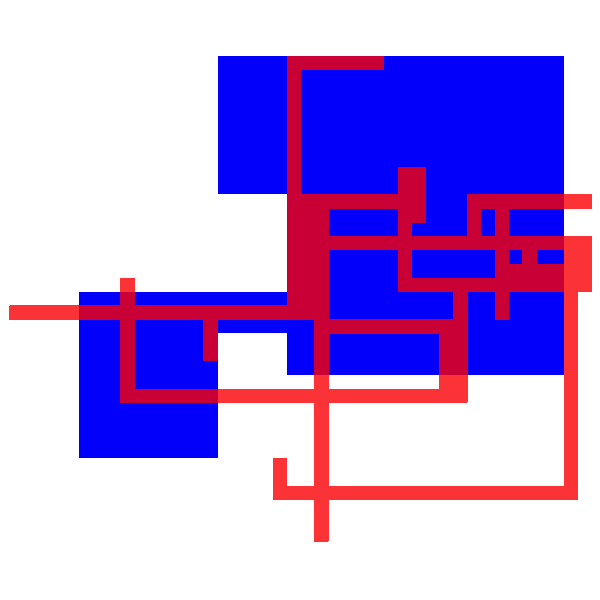
\includegraphics[width=\linewidth]{multilevel_digger}
	\caption{Multilevel map which floors have different topologies.}
	\label{fig:multilevel_digger}
 	\end{subfigure}
 	\hfill
  	\begin{subfigure}[t]{0.45\linewidth}
    			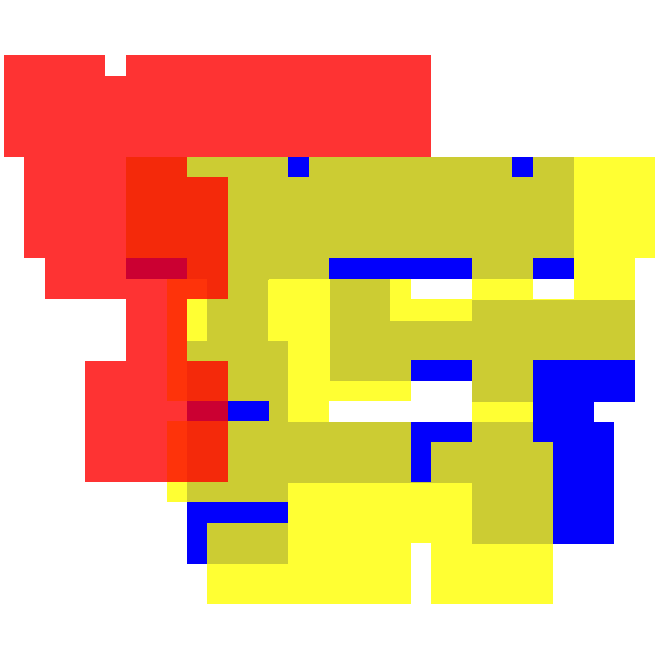
\includegraphics[width=\linewidth]{multilevel_divisive}
	\caption{Multilevel map which floors share the same topology.}
	\label{fig:multilevel_divisive}
  	\end{subfigure}
  	\hfill
\caption{Two multilevel maps.}
\end{figure}

\subsubsection{All-Black Multi-Level Map Manager}

The \<All-Black Multi-Level Map Manager> is used to decode multi-level maps saved in All-Black format. If no stairs are found among the objects, it employs the \<Stairs Generator> to position them.

% MAP GENERATOR %

\subsection{The Map Generator}

The \<Map Generator> controls the generation of the map. Each version of the \<Map Generator> defines a different \<map topology> depending on the used generation algorithm and on how its parametric settings are tuned. Some of these settings are shared by all the versions, whereas some of them are version-specific.

\par

The shared settings are used to define the size of the map and its encoding, to define the objects and to impose some constraints on their positioning:

\begin{itemize}
\item \<Width>: the number of rows of the matrix that represents the map.
\item \<Height>: the number of columns of the matrix that represents the map.
\item \<ObjectToObjectDistance>: the minimum number of cells that must separate two objects. 
\item \<ObjectToWallDistance>: the minimum number of cells that must separate an object and a wall.
\item \<BorderSize>: the width of the border placed all around the map once it has been generated, expressed in number of cells.
\item \<RoomChar>: the character used to represent a clear cell where the player can walk.
\item \<WallChar>: the character used to represent a filled cell where the player cannot walk.
\item \<MapObjects>: a list of the objects that must be placed in the map.
\end{itemize}

\noindent The objects contained in \<MapObjects> can represent spawn points, resources or decoration. They have the following properties:

\begin{itemize}
\item \<ObjectChar>: the character used to represent the object.
\item \<NumObjPerMap>: the number of objects of that kind that must be placed in the map.
\item \<PlaceAnywhere>: if this value is set to true, the restriction on the distance from the walls is ignored.
\item \<PositioningMode>: the algorithm used to position the object in the map.
\end{itemize}

\noindent The framework provides three different algorithms to position the objects inside the map:

\begin{itemize}
\item \<Rain>: positions the objects selecting random cells from the ones that are empty and satisfy the \<ObjectToWallDistance> constraint.
\item \<Rain Shared>: positions the objects selecting random cells from the ones that are empty and satisfy the \<ObjectToWallDistance> constraint and the \<ObjectToObjectDistance> constraint on the objects that have been placed using \<Rain Shared>.
\item \<Rain Distanced>: positions the objects selecting random cells from the ones that are empty and satisfy the \<ObjectToWallDistance> constraint and the \<ObjectToObjectDistance> constraint on the objects with the same \<ObjectChar>.
\end{itemize}

All of the following versions of the \<Map Generator> are deterministic, since they require a \<seed> value as input that constrains the output to a specific map.

% CELLULAR GENERATOR %

\subsubsection{Cellular Generator}

The \<Cellular Generator> employs a parametric \<cellular automaton>\footnote{A \<cellular automaton> consists of a grid of cells, each in one of a finite number of states, such as on and off. For each cell, a set of cells called its neighborhood is defined, usually composed by the ones that share at least one vertex with it (referred as \<8-neighbors>). Given the current state of the grid, a new generation is created, according to some fixed rule that determines the new state of each cell depending on the current state of the cell and of its neighbors.} to generate a natural looking map. 

\par

The algorithm starts by filling some tiles of the map selected at random, then it applies the cellular automaton for a certain number of generations and finally it performs some refinements (for more details, see algorithm \ref{alg:cellular}). The resulting topology depends on the following parameters:

\begin{itemize}
\item \<RandomFillPercent>: the percentage of tiles that are randomly filled during the initialization of the algorithm. High values promote narrow spaces, small values promote wide areas.
\item \<SmoothingInteration>: the number of generations the cellular automaton is ran for. High values penalize small features and make the walls smoother. 
\item \<NeighbourTileLimitLow>: the maximum number of neighbors a cell must have to became empty. Its value must be lesser or equal than the one of \<NeighbourTileLimitHigh>. The map becomes noisier the more they diverge.
\item \<NeighbourTileLimitHigh>: the minimum number of neighbors a cell must have to became filled.
\item \<WallThresholdSize>: the minimum number of cells that an isolated filled region must include to not be deleted. High values penalize small filled regions.
\item \<RoomThresholdSize>: the minimum number of cells that an isolated void region must include to not be deleted. High values penalize small empty regions.
\item \<PassageWidth>: the width of a passage connecting two different areas, expressed in number of cells.
\end{itemize}

\noindent Figure \ref{fig:cellulars} shows how these parameters influence the topology of a map.

\par

The \<Cellular Generator> can perform import and export using the text representation.

% DIVISIVE GENERATOR %

\subsubsection{Divisive Generator}\label{sssec:digger}

The \<Divisive Generator> employs a \<binary space partitioning algorithm> to generate a man-made looking map.

\par

The algorithm starts by obtaining partitions of the map by recursively dividing it in two sides of random size along one of the axes, then it selects some of these partitions as rooms and finally it connects them with corridors (for more details, see algorithm \ref{alg:divisive}). The resulting topology depends on the following parameters:

\begin{itemize}
\item \<RoomDivideProbability>: probability of a partition being divided again. High values promote small rooms.
\item \<MapRoomPercentage>: minimum percentage of tiles of the map that must be empty. High values promote close rooms separated by walls, low values promote distant rooms connected by corridors.
\item \<DivideLowerBound>: minimum division point expressed as percentage of the dimension of the room.
\item \<DivideUpperBound>: maximum division point expressed as percentage of the dimension of the room.
\item \<MinimumRoomDimension>: minimum width expressed in number of cells that a partition must have to be divided again. High values promote large rooms.
\item \<MinimumDepth>: the minimum number of recursive divisions that each partition must have experienced.
\item \<PassageWidth>: the width expressed in number of cells of the corridors connecting the rooms.
\item \<MaxRandomPassages>: the number of additional corridors to place, if possible, once that all the rooms are connected.
\end{itemize}

\noindent Figure \ref{fig:divisives} shows how these parameters influence the topology of a map.

\par

The \<Divisive Generator> can perform both import and export using the text representation, whereas the All-Black format is used only for export. The latter matches perfectly with this generator, since both are based on the concept of rooms and corridors.

% DIGGER GENERATOR &

\subsubsection{Digger Generator}

The \<Digger Generator> employs a simple algorithm to generate a man-made looking map.

\par

The algorithm is iterative and its state is defined by the current cell and by the current direction, that together with a randomly selected action determine the next cell that the algorithm is going to visit. Starting from the central cell of a filled map, at each iteration the algorithm empties the current cell and randomly decides if moving forward, turning left, turning right, jumping to a random visited cell or placing a flight of stairs, if controlled by a \<Multi-Level Generator>. The algorithm stops when a certain percentage of cells has been emptied. The resulting topology depends on the following parameters:

\begin{itemize}
\item \<ForwardProbability>: probability of moving forward in the next iteration. High values promote long corridors. 
\item \<LeftProbability>: probability of moving leftward in the next iteration. High values promote wide areas. 
\item \<RightProbability>: probability of moving rightward in the next iteration. High values promote wide areas. 
\item \<VisitedProbability>: probability of jumping to a visited cell in the next iteration. High values promote a more complex topology. 
\item \<StairProbability>: probability of placing a flight of stairs.
\item \<RoomPercentage>: percentage of tiles of the map that must be empty.
\end{itemize}

\noindent Figure \ref{fig:diggers} shows how these parameters influence the topology of a map.

\par

The \<Digger Generator> can perform both import and export using the text representation, whereas its own All-Black format is used only for import.

% GENERATORS ALGORITHMS AND IMAGES  %

\begin{algorithm}[tp]
\SetAlgoLined
\caption{Cellular generation algorithm.}
\algorithmfootnote{This algorithm is a modified version of the one proposed by Sebastian Lague\cite{lague}.}
\label{alg:cellular}

\For{every cell in the map}{
	empty the current cell\;
}

\While{percentage of filled cells $<$ RandomFillPercent} {
	select a random cell\;
	fill the selected cell\;
}

\For{generation from 0 to SmoothingIterations} {
	\For{every cell in the map}{
		count the 8-neighbors of the cell\;
		\If{8-neighbors  count $>$ NeighbourTileLimitLow}{
  			mark the current cell as filled for the next generation\;
   		}
		\If{8-neighbors  count $<$ NeighbourTileLimitHigh }{
  			mark the current cell as empty for the next generation\;
   		} 
	}
	update the map to the next generation\;
}

\For{every isolated region of empty cells}{
	\If{\#cells in the region $<$ RoomThresholdSize}{
		fill all the cells in the region\;
	}
}

\For{every isolated region of filled cells}{
	\If{\#cells in the region $<$ WallThresholdSize}{
		empty all the cells  in the region\;
	}
}

connect all the regions composed by empty cells\;
place the objects\;

\end{algorithm}

\begin{figure}[tp]
	\centering
  	\begin{subfigure}[t]{0.315\linewidth}
		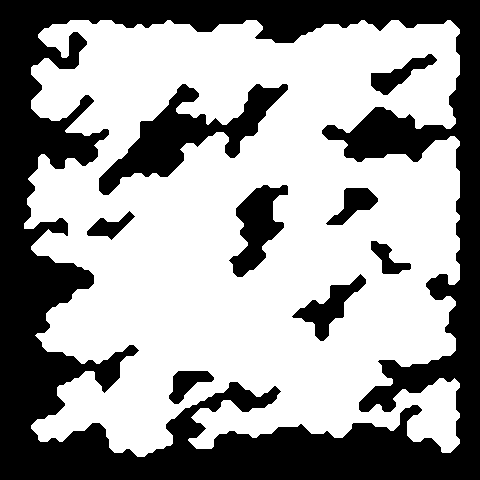
\includegraphics[width=\linewidth]{cellular_default}
     		\caption{Cellular map generated with the default settings.}
 	\end{subfigure}
 	\hfill
  	\begin{subfigure}[t]{0.315\linewidth}
    		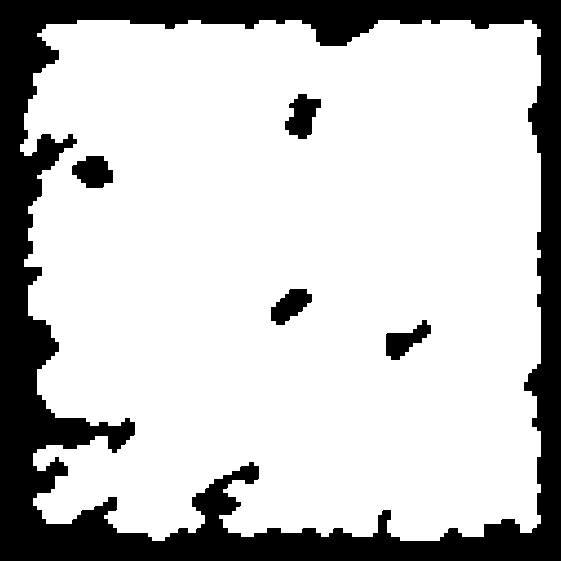
\includegraphics[width=\linewidth]{cellular_rfp40}
    		\caption{Cellular map generated with $Ran\-dom\-Fill\-Per\-cent = 40\%$.}
  	\end{subfigure}
  	\hfill
	\begin{subfigure}[t]{0.315\linewidth}
    		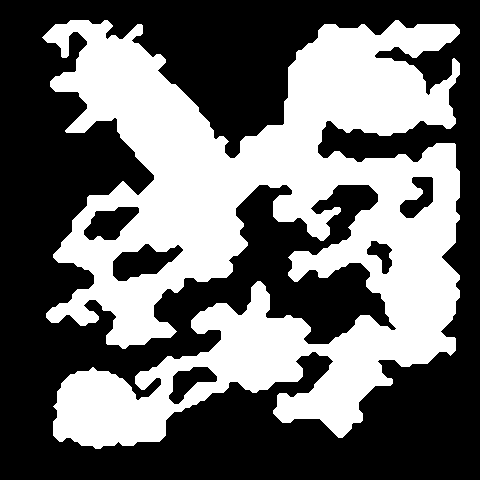
\includegraphics[width=\linewidth]{cellular_rfp50}
    		\caption{Cellular map generated with $Ran\-dom\-Fill\-Per\-cent = 50\%$.}
  	\end{subfigure}
  	
  	\begin{subfigure}[t]{0.315\linewidth}
		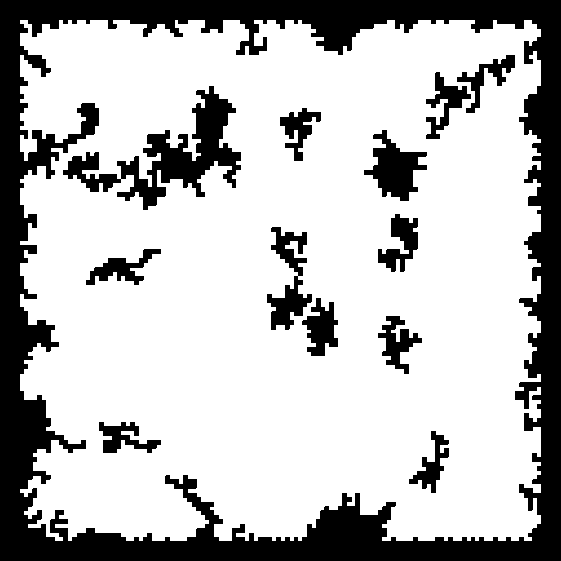
\includegraphics[width=\linewidth]{cellular_si0}
     		\caption{Cellular map generated with $Smooth\-ing\-It\-er\-a\-tions = 0$.}
 	\end{subfigure}
  	\hfill
  	\begin{subfigure}[t]{0.315\linewidth}
    		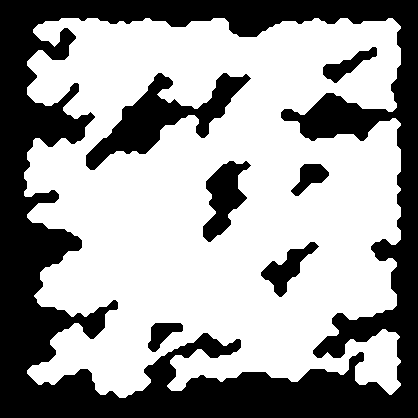
\includegraphics[width=\linewidth]{cellular_si3}
     		\caption{Cellular map generated with $Smooth\-ing\-It\-er\-a\-tions = 3$.}
  	\end{subfigure}
  	\hfill
  	\begin{subfigure}[t]{0.315\linewidth}
    		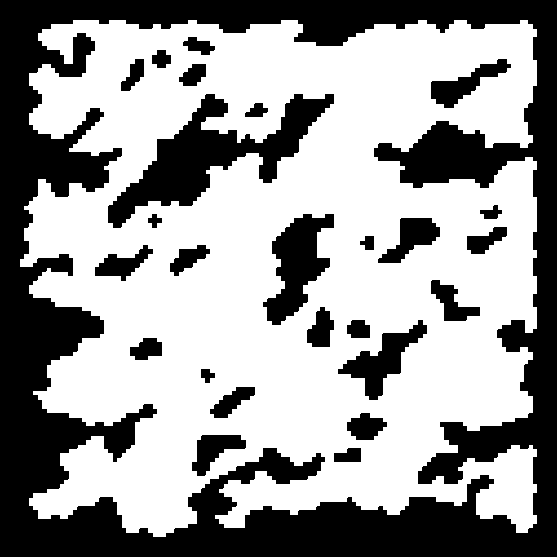
\includegraphics[width=\linewidth]{cellular_wts5}
     		\caption{Cellular map generated with $Wall\-Thresh\-old\-Size = 5$.}
  	\end{subfigure}	
	\caption[Six maps generated by the Cellular Generator using ``\<ANotSoRandomSeed>'' as seed, but different settings.]{Six maps generated by the Cellular Generator using ``\<ANotSoRandomSeed>'' as seed, but different settings. By default, the Cellular Generator has \<RandomFillPercent> set to $45\%$, \<SmoothingIterations> set to $2$,  \<NeighbourTileLimitHigh> set to $4$,  \<NeighbourTileLimitLow> set to $4$,  \<WallThresholdSize> set to $40$ and \<RoomThresholdSize> set to $100$.}
	\label{fig:cellulars}
\end{figure}

\begin{algorithm}[tp]
\SetAlgoLined
\caption{Divisive generation algorithm.}
\label{alg:divisive}

\For{every cell in the map}{
	fill the current cell\;
}

initialize the partitions list\;
DivideRoom(map, 0)\;

\While{percentage of empty tiles $<$ MapRoomPercentage}{
	extract a partition from the partitions list at random\;
	make the partition a room\;
	empty the tiles in the room\;
}

connect the rooms; 

\While{all the rooms are not directly connected \And \#placed additional corridors $<$ MaxRandomPassages}{
	add an additional corridor between two rooms selected at random;
}

place the objects\;

\hrulefill

\SetKwProg{Fn}{Function}{ is}{end}
\Fn{DivideRoom(section, depth)}{
	\eIf{(true with probability roomDivideProbability \And partition width $>$  minimumDividableRoomDimension \And partition heigth $>$ minimumDividableRoomDimension) \Or depth $<$  minimumDepth} {
		\eIf{previous division was horizontal} {
 			perform a random vertical division between \<divideLowerBound> and \<divideUpperBound>\;
		} {
 			perform a random horizontal division between \<divideLowerBound> and \<divideUpperBound>\;
		}
		DivdeRoom(first sub-section, depth + 1)\;
		DivdeRoom(second sub-section, depth + 1)\;
	}{
		add the partition to the partitions list;
	}	
}

\end{algorithm}

\begin{figure}[tp]
	\centering
  	\begin{subfigure}[t]{0.315\linewidth}
		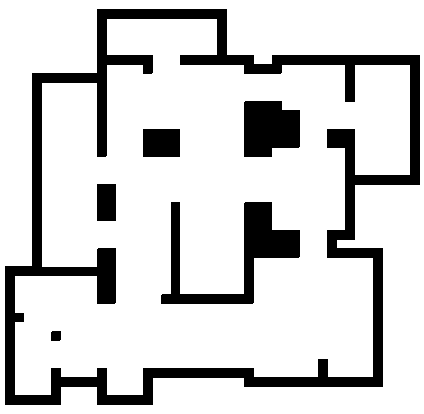
\includegraphics[width=\linewidth]{divisive_default}
     		\caption{Divisive map generated with the default settings.}
 	\end{subfigure}
	\hfill
  	\begin{subfigure}[t]{0.315\linewidth}
    		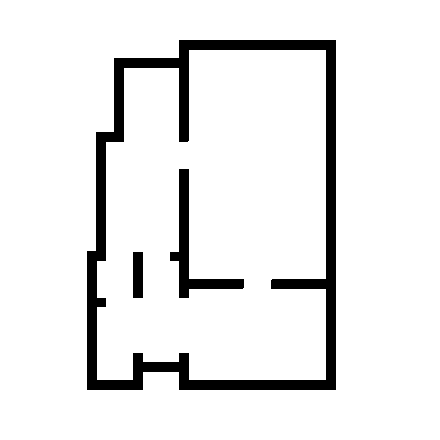
\includegraphics[width=\linewidth]{divisive_rdp20}
    		\caption{Divisive map generated with $Room\-Di\-vide\-Prob\-a\-bil\-i\-ty = 20\%$.}
  	\end{subfigure}
	\hfill
  	\begin{subfigure}[t]{0.315\linewidth}
    		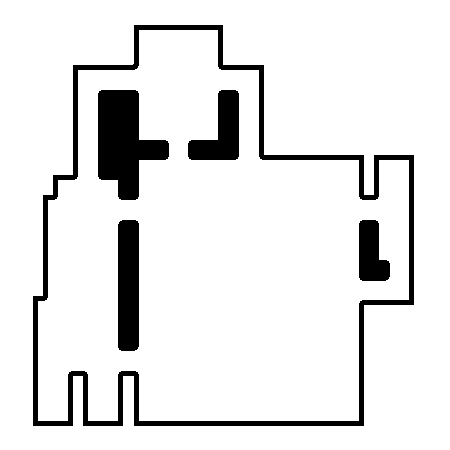
\includegraphics[width=\linewidth]{divisive_md1}
    		\caption{Divisive map generated with $Min\-i\-mum\-Depth = 1$.}
  	\end{subfigure}
  	
  	\begin{subfigure}[t]{0.315\linewidth}
		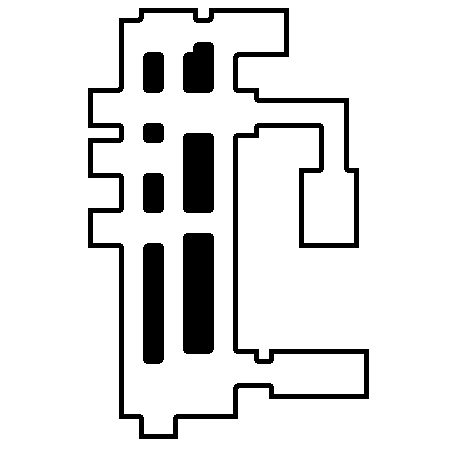
\includegraphics[width=\linewidth]{divisive_md8}
     		\caption{Divisive map generated with $Min\-i\-mum\-Depth= 8$.}
 	\end{subfigure}
 	\hfill
  	\begin{subfigure}[t]{0.315\linewidth}
    		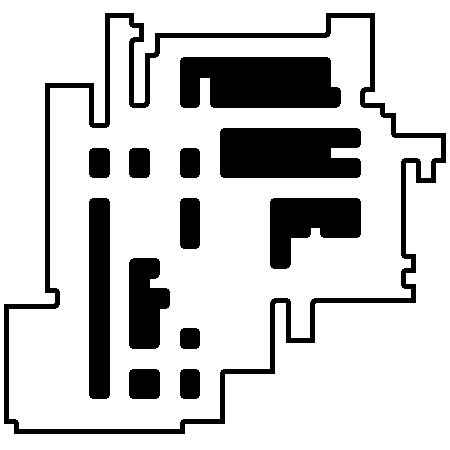
\includegraphics[width=\linewidth]{divisive_mrd1}
     		\caption{Divisive map generated with $Min\-i\-mum\-Room\-Di\-men\-sion = 1$.}
  	\end{subfigure}
	\hfill
  	\begin{subfigure}[t]{0.315\linewidth}
    		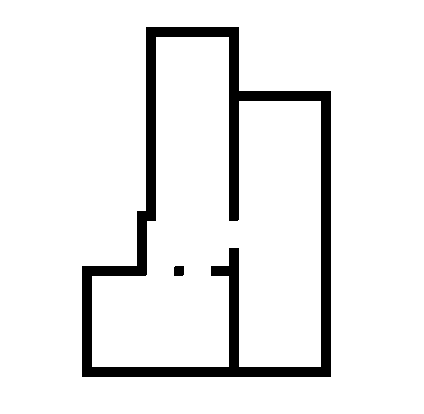
\includegraphics[width=\linewidth]{divisive_mrd7}
     		\caption{Divisive map generated with $Min\-i\-mum\-Room\-Di\-men\-sion = 7$.}
  	\end{subfigure}	
	\caption[Six maps generated by the Divisive Generator using ``\<AModeratelyRandomSeed>'' as seed, but different settings.]{Six maps generated by the Divisive Generator using ``\<AModeratelyRandomSeed>'' as seed, but different settings. By default, the Cellular Generator has \<Room\-Di\-vide\-Prob\-a\-bil\-i\-ty> set to $80\%$, \<Map\-Room\-Per\-cent\-age> set to $90\%$,  \<Di\-vide\-Low\-er\-Bound> set to $10\%$,  \<Di\-vide\-Up\-per\-Bound> set to $90\%$,  \<Min\-i\-mum\-Room\-Di\-men\-sion> set to $3$, \<Min\-i\-mum\-Depth> set to $4$, \<Pas\-sage\-Width> set to $3$ and \<Max\-Ran\-dom\-Pas\-sages> set to $12$.}
	\label{fig:divisives}
\end{figure}

\begin{figure}[tp]
\centering
\begin{subfigure}[t]{0.48\linewidth}
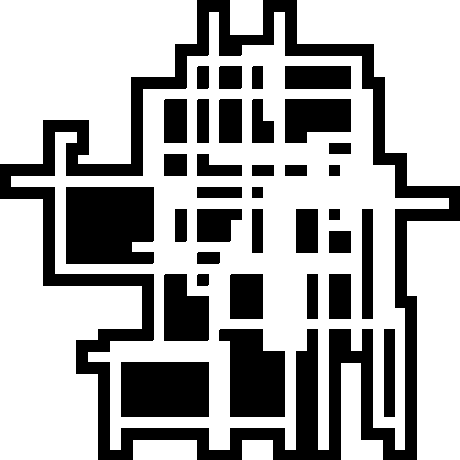
\includegraphics[width=\linewidth]{digger_default}
\caption{Digger map generated with the default settings.}
\end{subfigure}
\hfill
\begin{subfigure}[t]{0.48\linewidth}
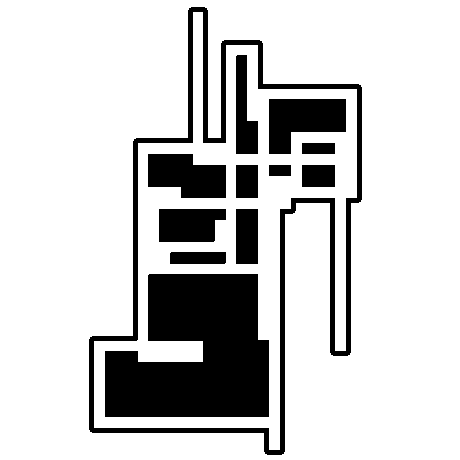
\includegraphics[width=\linewidth]{digger_roomp20}
\caption{Digger map generated with $Room\-Per\-cent\-age = 20\%$.}
\end{subfigure}

\begin{subfigure}[t]{0.48\linewidth}
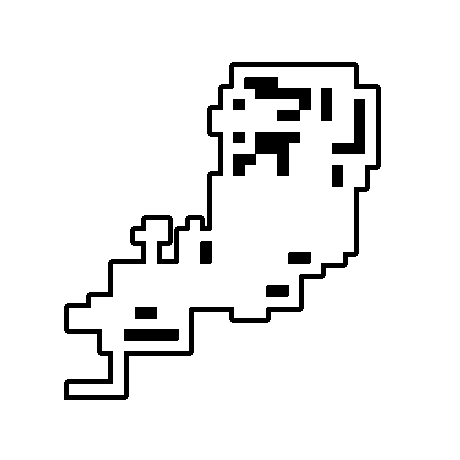
\includegraphics[width=\linewidth]{digger_fp60}
\caption{Digger map generated with $For\-ward\-Prob\-a\-bil\-i\-ty = 60\%$, $Right\-Prob\-a\-bil\-i\-ty = 19\%$ and $Left\-ward\-Prob\-a\-bil\-i\-ty = 19\%$.}
\end{subfigure}
\hfill
\begin{subfigure}[t]{0.48\linewidth}
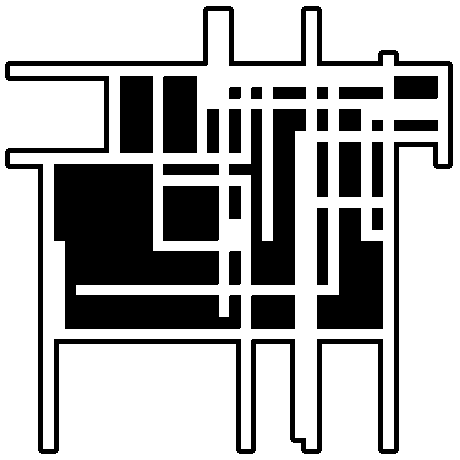
\includegraphics[width=\linewidth]{digger_fp96}
\caption{Digger map generated with $For\-ward\-Prob\-a\-bil\-i\-ty = 96\%$, $Right\-Prob\-a\-bil\-i\-ty = 1\%$ and $Left\-ward\-Prob\-a\-bil\-i\-ty = 1\%$.}
\end{subfigure}
\caption[Four maps generated by the Digger Generator using ``\<AFairlyRandomSeed>'' as seed, but different settings.]{Four maps generated by the Digger Generator using ``\<AFairlyRandomSeed>'' as seed, but different settings. By default, the Digger Generator has \<For\-ward\-Prob\-a\-bil\-i\-ty> set to $90\%$, \<Left\-Prob\-a\-bil\-i\-ty> set to $4\%$, \<Right\-Prob\-a\-bil\-i\-ty> set to $4\%$, \<Vis\-it\-ed\-Prob\-a\-bil\-i\-ty> set to $2\%$, \<Stair\-Prob\-a\-bil\-i\-ty> set to $0\%$ and \<Room\-Per\-cent\-age> set to $50\%$.}
\label{fig:diggers}
\end{figure}

% ALL-BLACK GENERATOR &

\subsubsection{All-Black Generator}

This simple generator parses inputs expressed in All-Black format, extracting rooms and corridors. If no objects are specified, it adds them to the map.

% STAIRS GENERATOR %

\subsection{The Stairs Generator}

The \<Stairs Generator> places stairs in the map after having analyzed it to find possible positions, but if stairs have already been placed by the \<Map Generator> (this happens with the \<Digger Generator>), it just validates them.

% MAP ASSEMBLER %

\subsection{The Map Assembler}

The \<Map Assembler> controls the assembly of the map. Each version of the Map Assembler corresponds to a different \<map appearance>.

% MESH ASSEMBLER %

\subsubsection{Mesh Assembler}

The \<Mesh Assembler> produces a 3D model of the map using an implementation of the \<marching squares algorithm>\footnote{\<Marching squares > is a computer graphics algorithm that generates contours for a \<two-dimensional scalar field>, i.e. a rectangular array of individual numerical values.} to generate three meshes: one for the floor, one for the walls and one for the ceiling. As it can be seen in figure \ref{fig:cellular_assembled}, the result is a natural-looking environment.

% PREFAB ASSEMBLER %

\subsubsection{Prefab Assembler}

The \<Prefab Assembler> produces a 3D model of the map by associating to each tile a specific 3D model, or \<prefab>, depending on the value of the tile and of its 8-neighbors (see figure \ref{fig:prefabs}). Figure \ref{fig:divisive_assembled} shows a map assembled with this algorithm.

\begin{figure}
\centering
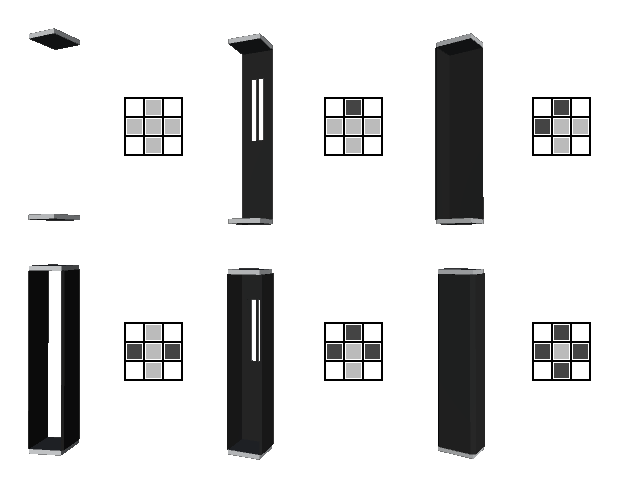
\includegraphics[width=0.95\linewidth]{prefabs}
\caption[Some prefabs and the masks they are associated to.]{Some prefabs and the masks they are associated to. Each model refers to the central cell of the corresponding mask. Green denotes empty cells, red denotes filled cell, half-green and half-red denotes cells that are ignored by the mask. The masks can be rotated to obtain all the possible configurations.}
\label{fig:prefabs}
\end{figure}

% MULTI-LEVEL PREFAB ASSEMBLER %

\subsubsection{Multi-Level Prefab Assembler}

Like the \<Prefab Assembler>, the \<Multi-Level Prefab Assembler> produces a 3D model of the map by combining prefabs, but it employs additional logic to manage the overlap of multiple floors. Figure \ref{fig:multi_assembled} shows a map assembled with this algorithm.

\begin{figure}
\centering
\begin{subfigure}[t]{0.48\linewidth}
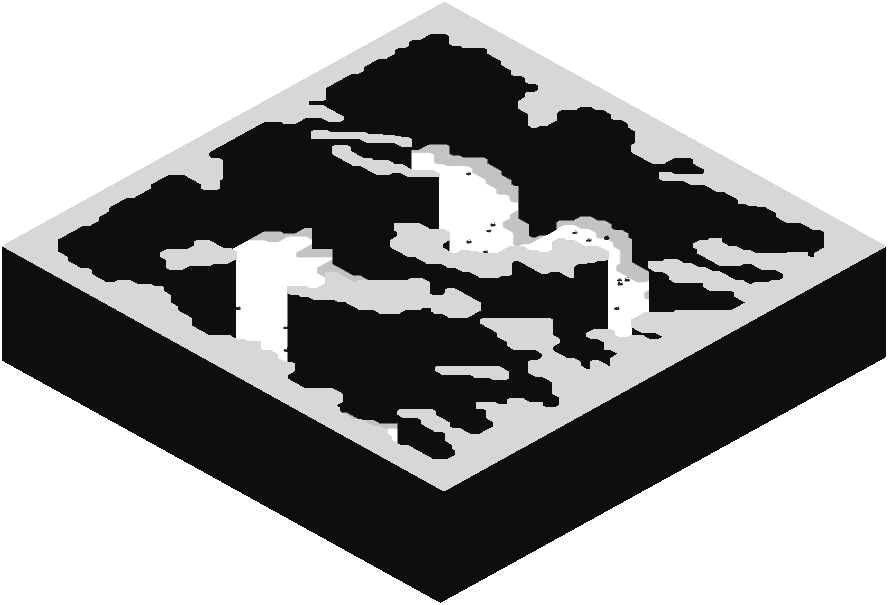
\includegraphics[width=\linewidth]{isometric_canyon}
\caption{Cellular map assembled with the \<Mesh Assembler>}
\label{fig:cellular_assembled}
\end{subfigure}
\hfill
\begin{subfigure}[t]{0.48\linewidth}
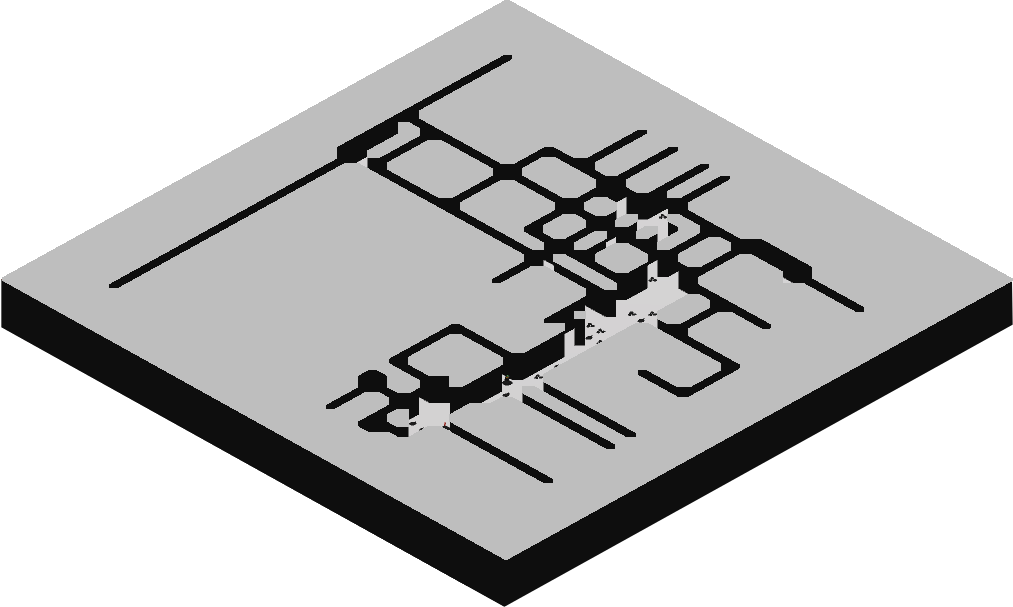
\includegraphics[width=\linewidth]{isometric_mine}
\caption{Digger map assembled with the \<Mesh Assembler>}
\label{fig:digger_assembled}
\end{subfigure}

\begin{subfigure}[t]{0.48\linewidth}
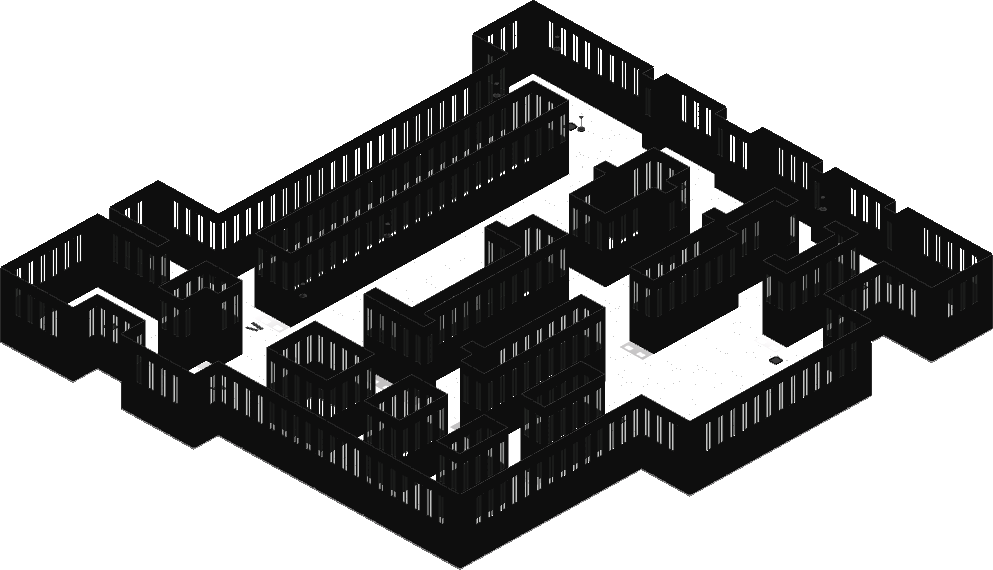
\includegraphics[width=\linewidth]{isometric_factory}
\caption{Divisive map assembled with the \<Prefab Assembler>}
\label{fig:divisive_assembled}
\end{subfigure}
\hfill
\begin{subfigure}[t]{0.48\linewidth}
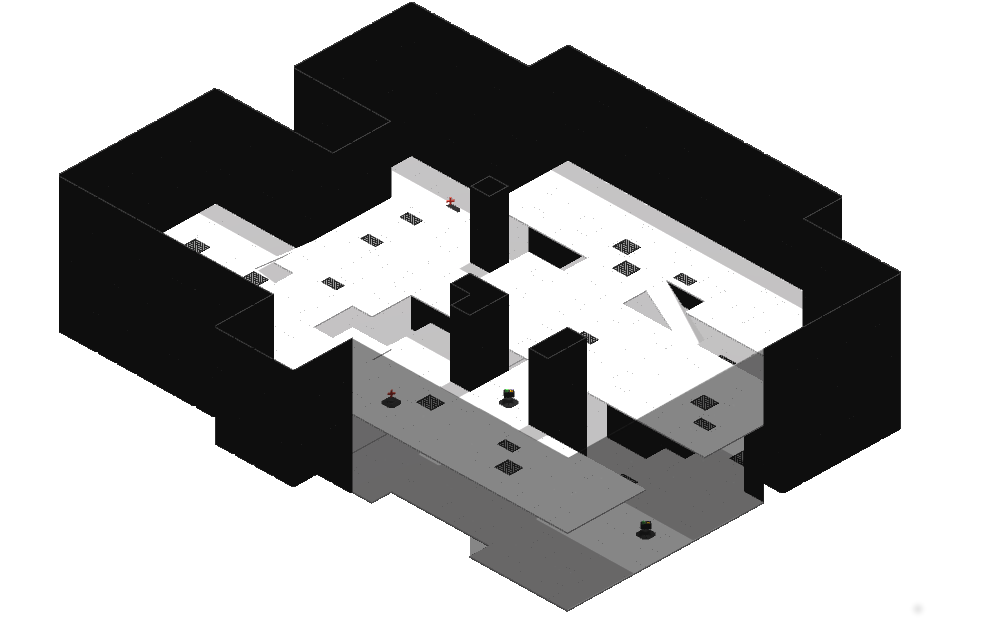
\includegraphics[width=\linewidth]{isometric_suburbs}
\caption{Multi-level map assembled with the \<Prefab Assembler>}
\label{fig:multi_assembled}
\end{subfigure}
\caption{Some possible combinations of generators and assemblers.}
\end{figure}

% SPAWN POINT MANAGER %

\subsection{The Spawn Point Manager}

The \<Spawn Point Manager> contains a list of all the spawn points displaced in the map, that is populated at the end of the \<Generation phase> by the \<Game Manager>. When the \<Game Manager> needs to spawn an entity, the \<Spawn Point Manager> provides a random spawn point from the ones that have not been used in a certain amount of time. If no spawn point meets this condition, the extraction is performed from the complete pool.

% OBJECT DISPLACER %

\subsection{The Object Displacer}

The \<Object Displacer> associates a character that represents neither a wall or a clear cell to the corresponding object, displacing it at the coordinates defined by its position in the map matrix. During this process, it populates a dictionary containing all the objects in the map divided by category, that is used by the \<Game Manager> to populate the list of spawn points used by the \<Spawn Point Manager>.

% EXPERIMENT MENAGER %

\subsection{The Experiment Manager}

The \<Experiment Manager> is a stand alone module that allows to create and manage the experiments used to perform user-based validation. Once that an experiment has been defined, the \<Experiment Manager> automatically assigns to the users the matches to play and collects the desired information.

\paragraph{Experiment definition}

\mbox{}\\

{\setlength{\parindent}{0cm}
An experiment is defined by a \<tutorial>, a list of \<studies> and a \<survey>.}

\par

The \<tutorial> is optional and consists in a match with a simple objective used to explain the commands to the user.

\par

The \<studies> are not optional and each one of them consists in a list of \<cases>. Each case contains a pool of maps and a single game mode, that is used to play the maps in the pool. The maps in the pool are the object of validation, whereas the game mode is the employed validation method.

\par

The \<survey> is optional and consists in a list of multiple-choice questions that are presented to the player at the end of the experiment.

\par

All these elements can be easily customized, as well as the number of test cases that an user has to play in a single experiment session, defined by the parameter \<CasesPerUsers>. The \<Experiment Manager> also allows to diagonally flip the maps, which is an useful method to avoid the rise of a bias due to memorization when the player is presented with different versions of the same map.

\paragraph{Experiment management}

\mbox{}\\

{\setlength{\parindent}{0cm}
Once that the experiment has been defined, it is ready to be played  by the users.}

\par

Each time that a user participates in the experiment, the \<Experiment Manager> selects the least played case of the least played study, in a round-robin fashion. This allows to have equally distributed data for each study and is possible thanks to the completion tracking provided by the \<Experiment Manager> itself. Then, for each case that the user is going to play, a pre-generated map is extracted from the pool and presented to the player as a match of the game mode specified by the case. In a complete experiment, the player will consecutively play the tutorial, one ore more matches and finally answer the survey.

\par

The experiment can be performed \<offline> or \<online>. In the former, the computed data and the experiment completion are stored locally, whereas in the latter, they are stored on a server. If the experiment is provided via an executable, then it is possible to configure it as \<offline>, \<online> or both, with the completion that is stored on a server and the computed data that is stored both locally and remotely. If the experiment is provided via a web build playable via browser, the only supported configuration is the \<online> one. 

\paragraph{Logging}

\mbox{}\\

{\setlength{\parindent}{0cm}
By default, the \<Experiment Manager> produces a complete log of each match, saving the following information:}

\begin{itemize}
\item \<MapInfo>: this field contains general information about the map featured in the match, as its name, its dimension, the size of its tiles and if it has been flipped.
\item \<GameInfo>: this field contains general information about the match, as the experiment name, the game mode and the duration.
\item \<SpawnLogs>: this field contains a list of all the spawn events. Each entry contains a timestamp, the coordinates of the spawn point and the name of the spawned entity.
\item \<PositionLogs>: this field contains a discretized list of the positions occupied by the player during the match, acquired with a given frequency. Each entry contains a timestamp, the coordinates of the player and the direction he is facing expressed in degrees.
\item \<ShotLogs>: this field contains a list of all the shots fired by the player. Each entry contains the same fields of the \<PositionLogs>, plus the identifier of the firing weapon, the number of projectiles in its magazine and its total available ammunition.
\item \<ReloadLogs>: this field contains a list of all the reloadings performed by the player. Each entry contains a timestamp, the identifier of the weapon that is being reloaded, the number of projectiles in its magazine and its total available ammunition, both before the reloading.
\item \<HitLogs>: this field contains a list of all the shots that hitted an entity. Each entry contains a timestamp, the coordinates of the hitted entity, the name of the hitted entity, the name of the hitter entity and the caused damage.
\item \<KillLogs>: this field contains a list of all the killings. Each entry contains a timestamp, the coordinates of the killed entity, the name of the killed entity and the name of the killer entity.
\end{itemize}

It is possible to customize the \<Experiment Manager> to have it compute and save specific metrics in a different log. Moreover, if the experiment includes a survey, the answers of the user are saved in a dedicated log.

\paragraph{Data retrieval}

\mbox{}\\

{\setlength{\parindent}{0cm}
The framework provides a simple interface for downloading the logs stored on the server. Since it is possible to set a limit on the dimension of logs which causes them to be split in multiple parts, the framework automatically performs merging and signals incomplete logs.
}

% ENTITIES %

\section{Entities}

The \<entities> are the \<agents> that take part in a match. All the entities share the following common features:

\begin{itemize}
\item \<TotalHealth>: the maximum number of health points of the entity, i.e. the quantity of damage the entity can receive before being destroyed.
\item \<Guns>: the guns associated to the entity.
\end{itemize}

The framework includes three different kind of agents:

\begin{itemize}
\item \<Player>: the entity that is controlled by the user. It can walk, jump, aim, deal and receive damage and pick resources.
\item \<Opponent>: this entity is similar to the one of the \<Player>, but in the current version of the framework it has no active logic, beside the one that controls its health.
\item \<Target>: this simple entity rotates in place. Besides receiving damage, it can harm the player thanks to the laser gun it can be equipped it. Figure \ref{fig:targets} shows different kind of targets.
\end{itemize}

\begin{figure}
\centering
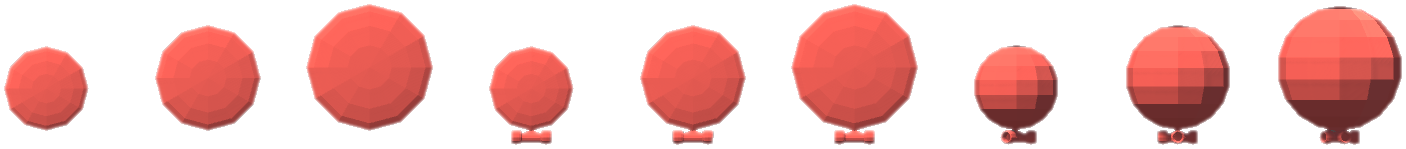
\includegraphics[width=0.95\linewidth]{targets}
\caption{Different ready-to-use target entities provided by the framework.}
\caption*{From the first to the third are simple targets, from the fourth to the sixth are targets equipped with two opposing laser guns, from the seventh to the ninth are``\<core>'' targets equipped with an increasing number of radial laser guns. The size of each target is proportional to its \<TotalHealth>.}
\label{fig:targets}
\end{figure}

% WEAPONS %

\section{Weapons}

The framework allows to easily define any kind of fire arm starting from a common parametric structure that characterizes the basic behavior of a gun with the following variables: 

\begin{itemize}
\item \<Damage>: the damage inflicted by a single projectile.
\item \<Dispersion>: the aperture of the cone-shaped projectile spread expressed in degree.
\item \<ProjectilePerShot>: the number of projectile emitted with one shot.
\item \<InfiniteAmmo>: tells if the gun has infinite ammunition.
\item \<ChargerSize>: the capacity of the gun magazine.
\item \<MaximumAmmo>: the maximum quantity of ammunition that can be carried for a specific gun.
\item \<ReloadTime>: the amount of time needed to reload the gun.
\item \<CooldownTime>:  the amount of time needed after a shot to fire again.
\item \<AimEnabled>: tells if the gun allows the player to aim.
\item \<Zoom>: the zoom provided by the scope when aiming.
\end{itemize}

\noindent This parametric approach allows to use the framework as a tool for user-based validation of procedurally generated weapons, that is another research field that has been explored in recent years \cite{ArmiProcedurali}.

\par 

The framework comes with three different categories of weapons already implemented.

\paragraph{Raycast guns}

\mbox{}\\

{\setlength{\parindent}{0cm}
\<Raycast guns> are weapons which projectiles have no \<time of flight>, but instantly hit the target once shot. The only additional parameter that this category introduces is \<Range>, which can be used to limit the reach of the weapon.
}

\par

There are three weapons of this category that the player can use:

\begin{itemize}
\item \<Assault Rifle>: a medium range weapon with a high fire rate, a capacious magazine and no dispersion which shots single medium damage projectiles. Figure \ref{fig:assault} shows its model and table \ref{tab:gunconfig} shows its parameters.
\item \<Shotgun>: a short range weapon with a slow fire rate, a small magazine and high dispersion which shots multiple low damage projectiles. Figure \ref{fig:shotgun} shows its model and table \ref{tab:gunconfig} shows its parameters.
\item \<Sniper Rifle>: a long range weapon with a slow fire rate, a small magazine and no dispersion which shots single high damage projectiles. It is equipped with a scope. Figure \ref{fig:sniper} shows its model and table \ref{tab:gunconfig} shows its parameters.
\end{itemize}

\paragraph{Projectile guns}

\mbox{}\\

{\setlength{\parindent}{0cm}
\<Projectile guns> are weapons that shoot projectiles with a limited flight speed. This category introduces two additional parameters:
}

\begin{itemize}
\item \<ProjectileLifetime>: if the projectile does not hit anything after this amount of time, it is destroyed.
\item \<ProjectileSpeed>: the speed of the projectile.
\end{itemize}

The only weapon of this category that the player can use is the \<Rocket Launcher>, a long range weapon with a slow fire rate, a small magazine and no dispersion which shots explosive projectiles. The projectiles of this weapon are slow and explode on impact, dealing an high damage that decreases radially from the center of the explosion. Figure \ref{fig:rocket} shows its model and table \ref{tab:gunconfig} shows its parameters.

\begin{figure}[p]
\centering
\begin{subfigure}[t]{0.48\linewidth}
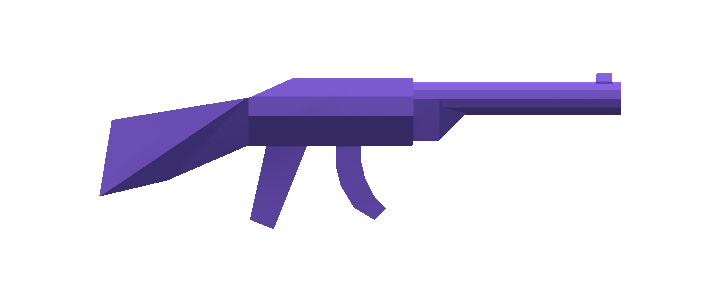
\includegraphics[width=\linewidth]{gun_assault}
\caption{The Assault Rifle.}
\label{fig:assault}
\end{subfigure}
\begin{subfigure}[t]{0.48\linewidth}
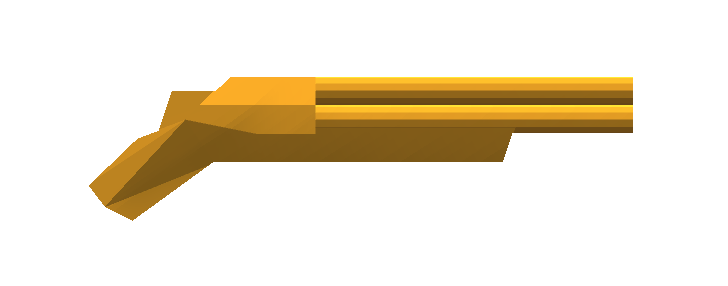
\includegraphics[width=\linewidth]{gun_shotgun}
\caption{The Shotgun.}
\label{fig:shotgun}
\end{subfigure}
\begin{subfigure}[t]{0.48\linewidth}
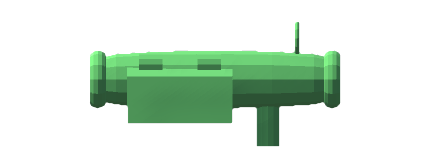
\includegraphics[width=\linewidth]{gun_rocket}
\caption{The Rocket Launcher.}
\label{fig:rocket}
\end{subfigure}
\begin{subfigure}[t]{0.48\linewidth}
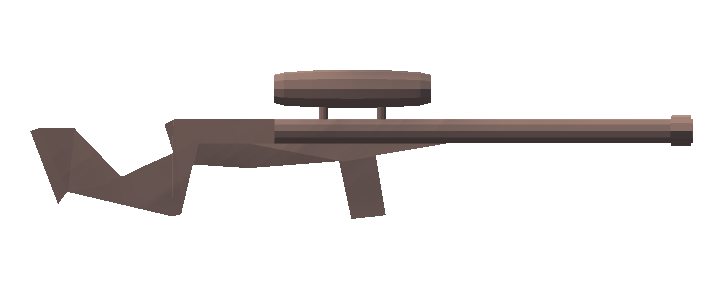
\includegraphics[width=\linewidth]{gun_sniper}
\caption{The Sniper Rifle.}
\label{fig:sniper}
\end{subfigure}
\caption{The weapons that the player can use.}
\end{figure}

\begin{table}[p]
\setlength\extrarowheight{2pt}
\begin{tabularx}{\textwidth}{|l|C|C|C|C|}
\cline{2-5}
\multicolumn{1}{c|}{}& Assault Rifle & Shotgun & Rocket Launcher & Sniper Rifle  \\
\hline
\<Damage> & 15  & 20  &  120 & 75  \\
\hline
\<Dispersion> & 0  & 7.5  & 0  & 0  \\
\hline
\<ProjectilesPerShot> &  1 &  5 & 1  & 1  \\
\hline
\<InfiniteAmmo> & false & false  & false &   false\\
\hline
\<ChargerSize> & 32  & 3  &  2 &  5 \\
\hline
\<MaximumAmmo> &  120 &  24 & 16  & 30  \\
\hline
\<ReloadTime> &  1 & 1  &  1 & 1  \\
\hline
\<CooldownTime> &  0.1 &  0.75 &  0.75 &  0.5 \\
\hline
\<AimEnabled> &  false & false  & false  & true  \\
\hline
\<Zoom> & 1  &  1 &  1 & 3  \\
\hline
\<LimitRange> & false  & true  &  - & false  \\
\hline
\<Range> &  - &  100 &  - &  - \\
\hline
\<ProjectileLifeTime> & -  & -  & 10  & -  \\
\hline
\<ProjectileSpeed> &  - &  - & 50 &  - \\
\hline
\end{tabularx}
\caption{Parametric configuration of the four weapons available to the player.}
    \label{tab:gunconfig}
\end{table}

\paragraph{Laser guns}

\mbox{}\\

{\setlength{\parindent}{0cm}
\<Laser guns> are not based on the same structure of the previous categories. Laser guns emit a continuous ray that deals damage over time to everything it touches. Their only configurable parameter is \<DPS> (\<damage per second>), i.e. the damage the the gun deals in a second when continuously hitting a target.
}

% OBJECTS %

\section{Objects}

Beyond \<decorations>, that are simple 3D models with no logic used to graphically enrich the map, the framework provides \<spawners>, i.e. objects that spawn a resource that can be collected by the entities. Once that the resource is collected, it disappears for an interval  of time defined by the parameter \<Cooldown>. The framework comes with two different \<spawners>:

\begin{itemize}
\item \<Health pack Spawner>: it spawns health packs, that partially restore the health of the entity. The healed amount of health is defined by \<RestoredHealth>.
\item \<Ammunition Spawner>: it spawns ammunition crates, that supply the entity with ammunition. \<SuppliedGuns> defines which guns the crates can supply, whereas \<AmmoAmounts> defines how many ammunition are provided to the entity for each supplied weapon.

\end{itemize}

% GAME MODES %

\section{Game modes}

The framework comes with three different game modes, that have been designed to highlight specific aspects of a multiplayer FPS. Each game mode is defined by a different version of the \<Game Manager>.

\subsection{Duel}

The \<Duel> game mode is a classic \<deathmatch> redistricted to two entities, with one of the two being the player. Each time that an entity eliminates the other one, it scores one point, whereas it loses one if it destroys itself by accident. When an entity has been eliminated, it \<respawns>\footnote{In video games, \<respawn> denotes the reappearing in a specific location, called \<spawn point>, of an entity which has been eliminated.} at a random spawn point. At the end of the match, which is marked by a time limit, the winner is the contender who has scored the highest number of points.

\par

Of the game modes that the framework provides, this one is the most complete, because it contains all the dynamics that characterize a multiplayer FPS match, and the most important, since it is the one that is usually used to perform validation in this research field.

\subsection{Target Rush}

\begin{figure}
\centering
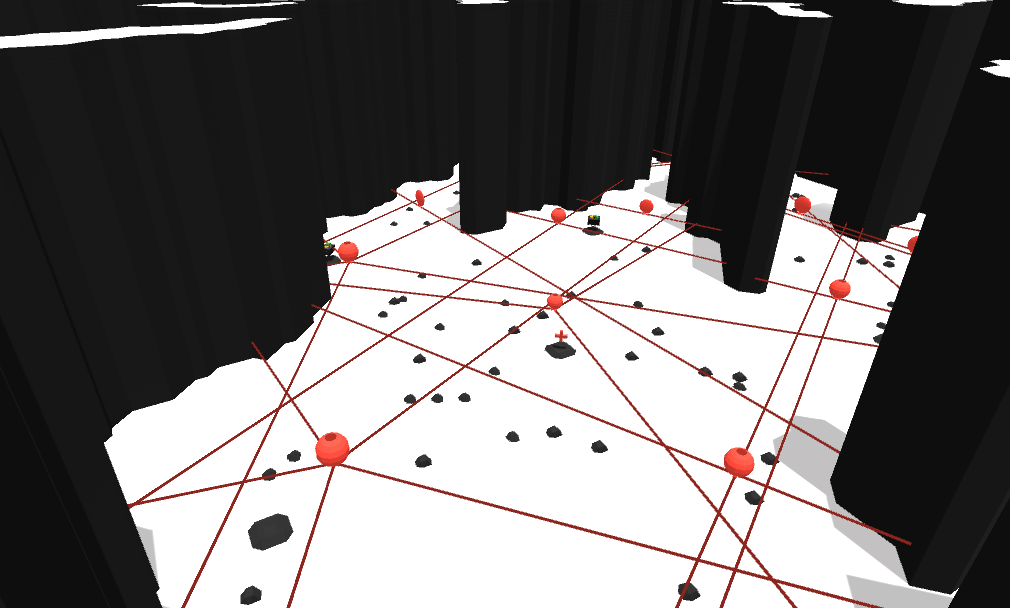
\includegraphics[width=0.95\linewidth]{rush20}
\caption{Targets equipped with laser guns in the final wave of a \<Target Rush> match.}
\label{fig:targets}
\end{figure}

In the \<Target Rush> game mode the player faces increasingly difficult waves of enemies, trying to obtain a score as high as possible before the end of the game, that is triggered by the player death or by the countdown hitting zero. The player earns points and additional time when he destroys an enemy or he completes a wave. The number of waves is parametric, as well as the content of each one. By default, this mode has twenty waves and uses targets as enemies, that start as harmless but became more and more numerous and dangerous with each wave (see figure \ref{fig:targets}). 

\par

This game mode has been designed to force the player to explore the map, through the research of enemies, health packs and ammunition, that quickly become indispensable as the match progresses.

\subsection{Target Hunt}

In the \<Target Hunt> game mode the player needs to find and eliminate a series of enemies in a given amount of time. The  enemies that the player is going to face are stored in a parametric list that is read circularly and are spawned one at a time, as soon as the previous one has been eliminated. To each enemy is assigned a score.

\par

This game mode has been designed to force the player to search a specific objective in the map.

\section{Summary}

In this chapter we analyzed the framework that we have developed to perform user-based validation, focusing on its structure, its components and its parametric nature.